\documentclass[aspectratio=169,t]{beamer}
\usepackage[utf8]{inputenc}
\usepackage[T1]{fontenc}
\usepackage[english]{babel}
\usepackage{hyperref}
\usepackage{tikz}

\usepackage{graphicx}
\usepackage{epstopdf}
\usepackage{multirow}

\usepackage{psfrag}
\usepackage{pgfplots}
\usepackage{framed}
\usepackage{xcolor}
\usepackage{booktabs}
\usepackage{caption}
\usepackage{epstopdf}
\usepackage{amsmath}
\usepackage{tabularx}
\usepackage[]{bookmark}
%\usepackage[3D]{movie15}
%\usepackage{media9}
\usepackage[binary-units,abbreviations]{siunitx}
\usepackage[textfont=normalsize, labelfont=normalsize, justification=centering]{subcaption}
\usepackage{marvosym}
\usepackage{calc}
\usepackage{color, colortbl}
\usepackage[]{svg} 
\usepackage[]{trfsigns} 
\usepackage[nomessages]{fp}
\usepackage[]{csquotes}\MakeOuterQuote{"}
\selectcolormodel{rgb}

\makeatletter
\def\beamer@calltheme#1#2#3{\def\beamer@themelist{#2}
	\@for\beamer@themename:=\beamer@themelist\do
	{\usepackage[{#1}]{\beamer@themelocation/#3\beamer@themename}}}
\def\usefolder#1{\def\beamer@themelocation{#1}}
\def\beamer@themelocation{}
\usefolder{theme}

\usetikzlibrary{matrix,
	decorations.pathreplacing,
	calc,
	positioning,
	external,
	3d,
	shapes,
	arrows,
	pgfplots.statistics}
\pgfplotsset{compat=1.16}
\tikzstyle{faunode}=[rounded corners, draw=faublue, fill=faublue!10,  align=center, inner sep=0.3cm, line width=0.4mm]
\tikzstyle{fauellipseFixedWidth}=[ellipse, draw=faublue, fill=faublue!10,  align=center, inner sep=0.3cm, line width=0.4mm, minimum width=3cm]
\tikzstyle{fauellipse}=[ellipse, draw=faublue, fill=faublue!10,  align=center, inner sep=0.3cm, line width=0.4mm]
\tikzstyle{fauarrow}=[draw=faublue,->, line width=0.4mm]
\tikzstyle{fauline}=[draw=faublue, line width=0.4mm]


\usepackage[backend=bibtex,sorting=none,doi=true,style=phys]{biblatex}
%\usepackage[]{biblatex}
\bibliography{./references}

% Themes:
%  - fau:          FAU theme
%  - fau-tf:       TechFak FAU theme
%  - fau-tf-lme:   TechFak LME FAU theme
%
% Options:
%  - image:        Cover image on title page
%  - plain:        Plain title page
%  - longtitle:    Title page layout for long title
\usetheme[longtitle]{fau-tf-lme}

% END of THEME SETTINGS
% --------------------------------------------------------------------------------------------------------------------------------------------------------------------------

\sisetup{
exponent-product =\ensuremath{{\,\cdot\,}}
}

% Enable semi-transparent animation preview
\setbeamercovered{transparent}
\setbeamertemplate{blocks}[rounded]
\captionsetup{labelformat=empty,labelsep=none, labelfont=normalsize, justification=centering}


\newcommand\Wider[2][1.0cm]{%
\makebox[\linewidth][c]{%
  \begin{minipage}{\dimexpr\textwidth+#1\relax}
  \raggedright#2
  \end{minipage}%
  }%
}


\let\origitem\item
\renewcommand{\item}{\normalfont\origitem}
\newcommand{\bluefat}[1]{\textcolor{faublue}{\textbf{#1}}}
\newcommand{\bolditem}{\normalfont\origitem\bfseries}
\newcommand{\question}{{\bf Question: }}
\newcommand{\answer}{{\bf Answer: }}
\newcommand{\myExample}{{\bf Example }}
\newcommand{\real}{\mbox{${\mathbb R}$}}
\definecolor{defColor}{rgb}{0.8,0.87,0.97}
\definecolor{defColorT}{rgb}{0,0,0}
\definecolor{defColorF}{rgb}{1,1,1}
\newenvironment{myDefinition}{%
	\def\FrameCommand{\fboxsep=\FrameSep{} \fcolorbox{defColorF}{defColor}}%
	\color{defColorT}\MakeFramed{\FrameRestore{}}}%
{\endMakeFramed}

% Title page
\title[Medical Engineering II]{Medical Engineering - Imaging Systems}
\author{Prof.\ Dr.-Ing.\ habil.\ Andreas Maier}
\date{SS 2021}
\institute{Pattern Recognition Lab (CS 5)}

\newcommand{\password}{\texttt{mt2\_ss21}}


\AtBeginSection[]{
	{
		\setbeamertemplate{footline}{}
		\begin{frame}[noframenumbering]{\insertsubtitle}
			 \tableofcontents[currentsection]
		\end{frame} 
	}
}
\AtBeginSubsection[]{
	{

		\setbeamertemplate{footline}{}
		\begin{frame}[noframenumbering]{\insertsubtitle}
			 \tableofcontents[currentsection, currentsubsection]
		\end{frame} 
	}
}


\newcommand{\abs}[1]{\ensuremath{\big\vert #1\big\vert}}

\usepackage{wrapfig}

\subtitle{Nuclear Medicine}

\AtBeginSection[]{
    {
        \setbeamertemplate{footline}{}
        \begin{frame}[noframenumbering]{\insertsubtitle}
         \large   \tableofcontents[currentsection]
        \end{frame} 
    }
}
\AtBeginSubsection[]{
    {

        \setbeamertemplate{footline}{}
        \begin{frame}[noframenumbering]{\insertsubtitle}
            \large \tableofcontents[currentsection, currentsubsection]
        \end{frame} 
    }
}

\begin{document}

\frame[plain]{\titlepage}

\section{Introduction}%
\label{sec:introduction}



% New introductory slide

\begin{frame}[c]{Tracer Principle}
    \begin{columns}[T]
        \column{0.5\textwidth}
        In 1935, Georg de Hevesy injected radioactive $^{32}$P into rats and found that it accumulated in bones. With this experiment, he proved that bones are living tissue and inadvertently invented a new field of functional imaging based on the \emph{tracer principle}.  \\[0.5cm]
        This method formed the basis for functional imaging of biological processes.

        \column{0.4\textwidth}
        \begin{centering}
            \includegraphics[width=0.4\textwidth]{images/deHevesy}\\
        \end{centering}
        {\scriptsize Georg de Hevesy ca. 1913. He probably would have been smiling, had he known he would win the Nobel Prize for chemistry $30$ years later. Source: Wikipedia}

    \end{columns}
\end{frame}



\begin{frame}{Functional Imaging I}
    \begin{center}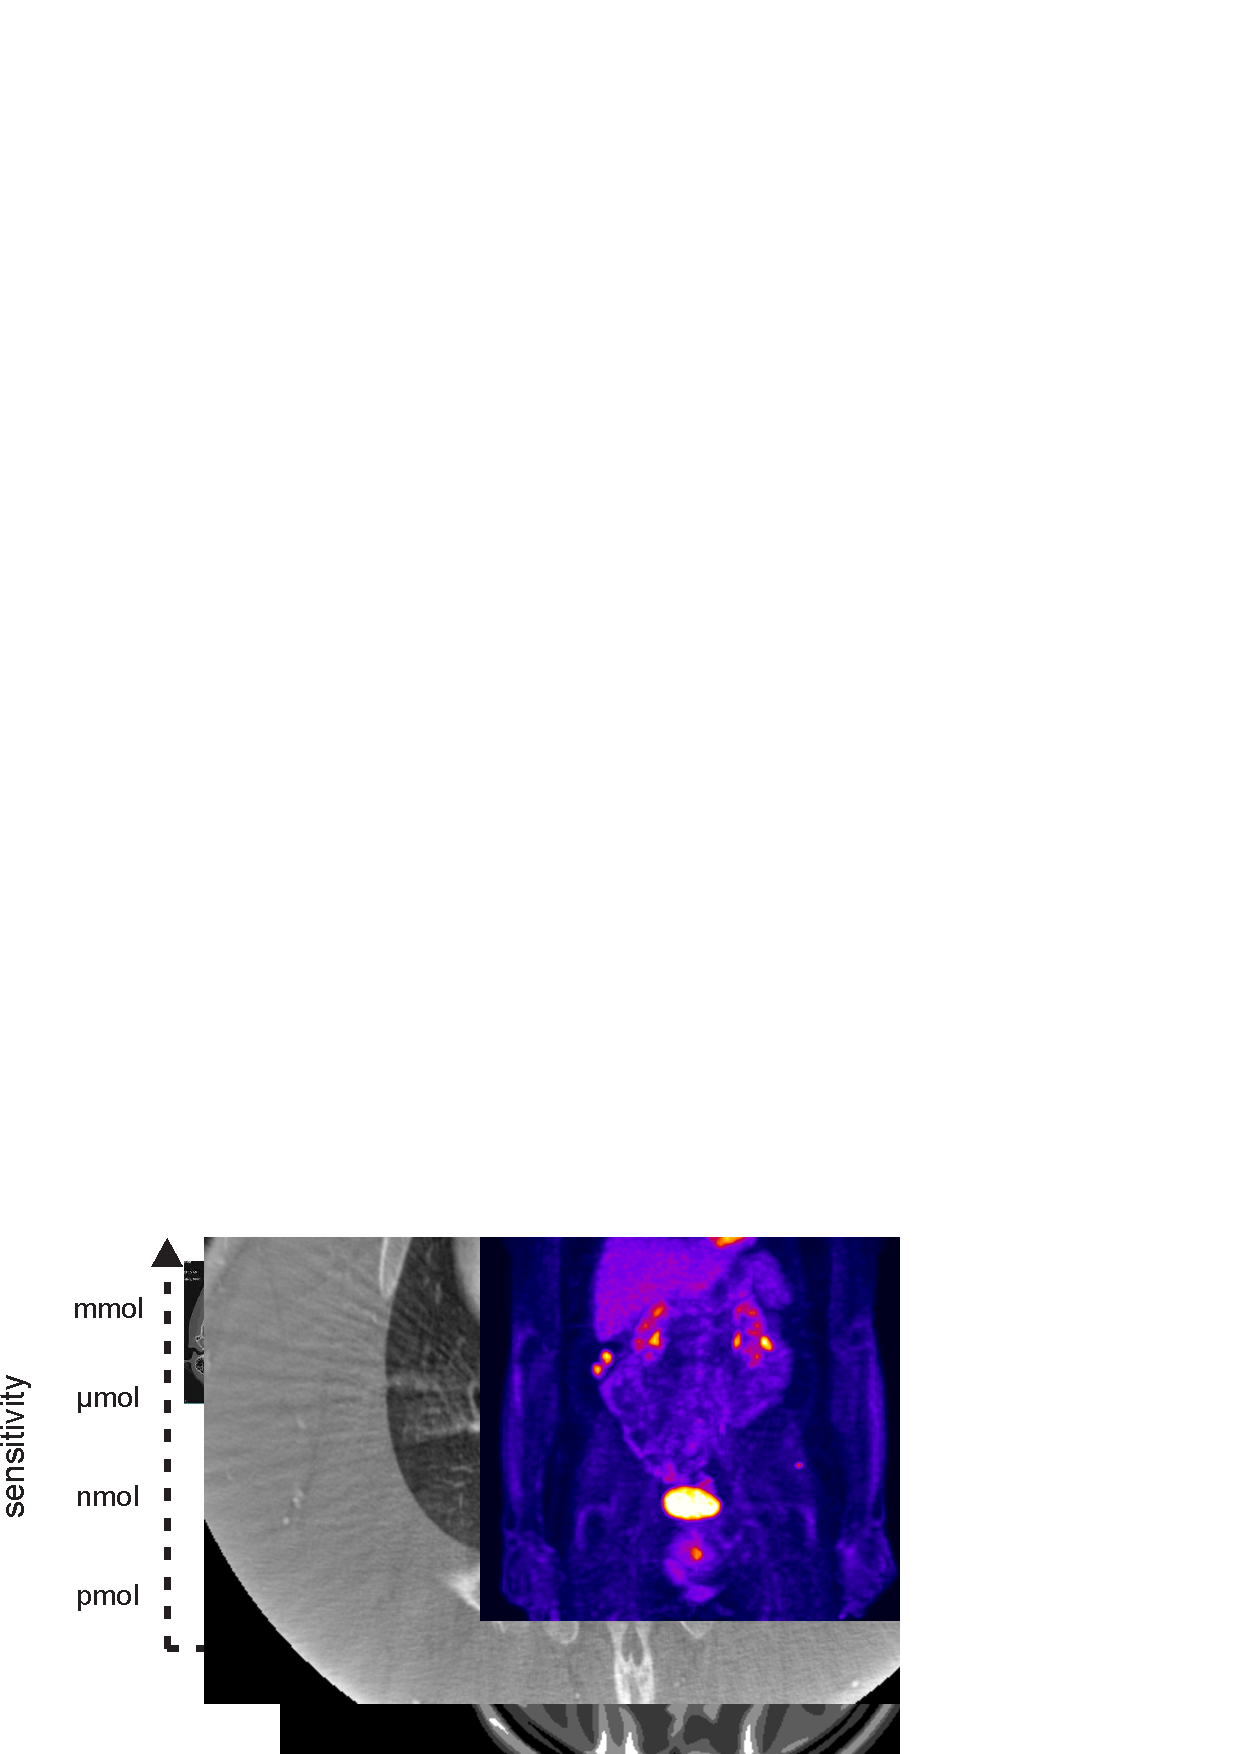
\includegraphics[height=0.7\textheight]{../00_motivation/Bilder/moletab.pdf}\\
        \begin{itemize}
            \item {Radiotracer administered and distributed in body based on pharmacokinetic properties.}\\
            \item {Used to image biological \emph{processes} as opposed to \emph{structures}}

        \end{itemize}
    \end{center}
\end{frame}


\begin{frame}{Functional Imaging II}
    \begin{center}%
        {
            \raggedright
            Isotope administration:\\
            \begin{itemize}
                \item{Injection}\\
                \item{Oral administration}\\
                \item{Inhalation}\\
            \end{itemize}

            Isotope distribution in patient's body driven by:\\
            \begin{itemize}
                \item{Perfusion}\\
                \item{Metabolism}\\
            \end{itemize}
        }
        \bigskip
        {\LARGE Goal is to image resulting activity distribution\\
            \bigskip
            {$\nu$}$(x,y,z,t)$}\\
    \end{center}
\end{frame}


\section{Physical Foundations}%
\label{sec:physical_foundations}




\begin{frame}{Isotopes}
    \vspace{-0.9cm}
    \begin{center}
        \begin{columns}[b, onlytextwidth]
            \begin{column}{0.3\textwidth}
                \begin{figure}
                    \begin{center}
                        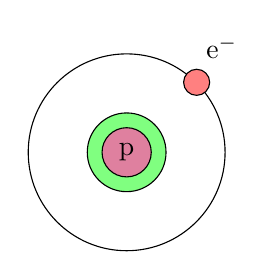
\begin{tikzpicture}[scale=1, transform shape]
                            \node (nucleus) [fill=green!50,draw,circle, minimum size=1cm] at (0,0) {};
                            \node (p) [fill=purple!50,draw,circle, minimum size=0.6cm] at (0,0) {p};
                            \node (radius) [draw,circle, minimum size=2.5cm] at (0,0) {};
                            \node (e) [draw,circle, fill=red!50, minimum size=0.2] at (radius.north east) {};
                            \node (elabel) [above right=0.0cm and 0.0cm of e.north]  {e${}^-$};
                        \end{tikzpicture}
                    \end{center}
                    \caption{\Large ${}_1^1$ H}
                \end{figure}
            \end{column}\begin{column}{0.3\textwidth}
                \begin{figure}
                    \begin{center}
                        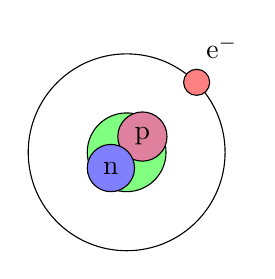
\begin{tikzpicture}[scale=1, transform shape]
                            \node (nucleus) [fill=green!50,draw,circle, minimum size=1cm] at (0,0) {};
                            \node (p) [fill=purple!50,draw,circle, minimum size=0.6cm] at (0.2,0.2) {p};
                            \node (p) [fill=blue!50,draw,circle, minimum size=0.6cm] at (-0.2,-0.2) {n};
                            \node (radius) [draw,circle, minimum size=2.5cm] at (0,0) {};
                            \node (e) [draw,circle, fill=red!50, minimum size=0.2] at (radius.north east) {};
                            \node (elabel) [above right=0.0cm and 0.0cm of e.north]  {e${}^-$};
                        \end{tikzpicture}
                    \end{center}
                    \caption{\Large ${}_2^1$ H}
                \end{figure}
            \end{column}\begin{column}{0.3\textwidth}
                \begin{figure}
                    \begin{center}
                        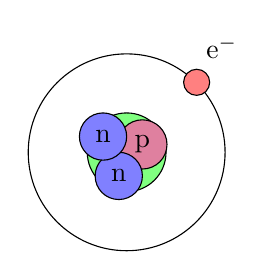
\begin{tikzpicture}[scale=1, transform shape]
                            \node (nucleus) [fill=green!50,draw,circle, minimum size=1cm] at (0,0) {};
                            \node (p) [fill=purple!50,draw,circle, minimum size=0.6cm] at (0.2,0.1) {p};
                            \node (p) [fill=blue!50,draw,circle, minimum size=0.6cm] at (-0.1,-0.3) {n};
                            \node (p) [fill=blue!50,draw,circle, minimum size=0.6cm] at (-0.3,0.2) {n};
                            \node (radius) [draw,circle, minimum size=2.5cm] at (0,0) {};
                            \node (e) [draw,circle, fill=red!50, minimum size=0.2] at (radius.north east) {};
                            \node (elabel) [above right=0.0cm and 0.0cm of e.north]  {e${}^-$};
                        \end{tikzpicture}
                    \end{center}
                    \caption{\Large ${}_3^1$ H}
                \end{figure}
            \end{column}
        \end{columns}

        \begin{center}
            \Huge{$^A_Z$X}
        \end{center}

        \vspace{0.4cm}
        \begin{itemize}
            \item[A:]  Mass Number = Number of nucleons in nucleus
            \item[X:]  Chemical element symbol
            \item[Z:] Atomic number = Number of protons in nucleus
        \end{itemize}
    \end{center}
\end{frame}


\begin{frame}[c]{Radioactive Decay}
    \raggedright
    Some isotopes have unstable combinations of particles in the nucleus and \emph{decay} into stable states.\\[0.25cm]
    The field of Nuclear Medicine takes advantage of particles released during transition for imaging and therapy. \\[0.25cm]
    Decay mechanisms include: \\
    \begin{itemize}
        \item $\alpha$ or $\beta$ decay
        \item Electron capture
        \item Isomer transition
        \item Spontaneous fission
    \end{itemize}

\end{frame}


\begin{frame}[c]{Ionizing Radiation}
    \begin{table}[ht]
        \begin{tabular}{|l | l | l| l|}
            \hline
            \textbf{Notation} & \textbf{Name}   & \textbf{Particle} & \textbf{Application} \\
            \hline
            $\gamma$          & Gamma radiation & Photons           & Diagnostics          \\
            \hline
            $\beta^-, e^-$    & Beta radiation  & Electrons         & Therapy              \\
            \hline
            $\beta^+,e^+$     & Beta radiation  & Positrons         & Diagnostics          \\
            \hline
            $p$               &                 & Protons           &                      \\
            \hline
            $n$               &                 & Neutrons          &                      \\
            \hline
            $\alpha$          & Alpha radiation & Helium nuclei     & Therapy              \\
            \hline
        \end{tabular}
    \end{table}
    %\bigskip
    %\begin{columns}[T, onlytextwidth]
    %\begin{column}{0.6\textwidth}\centering
    %\includegraphics[width=0.3\textwidth]{images/Radioaktiv}\\
    %\end{column}
    %\begin{column}{0.5\textwidth}
    %\includegraphics[width=0.3\textwidth]{images/Shielding}\\
    %{\scriptsize Source: Wikipedia}
    %\end{column}
    %\end{columns}

\end{frame}



%\begin{frame}{Radioactive Decay}
%	\begin{table}[ht]
%	\begin{tabular}{l | c l}
%	\hline
%	$\alpha$ Decay & $^{226}_{88}Ra \longrightarrow ^{222}_{82}Rn + ^4_2\alpha + \gamma$\\
%	\hline
%	$\beta^-$ Decay & $^{131}_{53}J \longrightarrow ^{131}_{54}Xe + e^- + \nu + (\gamma)$ \\
%			     & $n \longrightarrow p + e^- + \nu$\\
%	\hline
%	$\beta^+$ Decay & $^{11}_6C \longrightarrow ^{11}_5B + e^+ + \nu + (\gamma)$\\
%	 & $p \longrightarrow n + e^+ + \nu$\\
%	\hline
%	Electron Capture & $^{201}_{81}Tl \longrightarrow ^{201}_{80}Hg^m$\\
%	 & $p + e \longrightarrow n$\\
%	\hline
%	Isomer Transition & $^{99m}Tc \longrightarrow  _{99}Tc + \gamma$\\
%	\hline
%	Spontaneous & $^{236}_{92} \longrightarrow  ^{99}_{42}Mo + ^{133}_{50}Sn + 4 ^0_6n$\\
%	Fission & \\
%	\hline
%	\end{tabular}
%	\end{table}
%\end{frame}

\begin{frame}{Decay Law}

    \begin{center}
        {\LARGE
            $S(t)=S_0 \cdot e^{-\lambda t}$\\
        }
        \bigskip
        $S(t)$ = Number of radionuclides at time t\\
        $S_0$ = Number of radionuclides at time t = 0\\
        $\lambda$ = Decay constant\\
        \bigskip\bigskip
        {\LARGE $t_{1/2} = \frac{ln 2}{\lambda}$ }\\
        \bigskip
        $t_{1/2}$ = Half life\\
    \end{center}
\end{frame}

\begin{frame}{Activity}
    \begin{center}
        Activity = Number of decays per time frame\\
        \bigskip
        {\LARGE
            $Q(t)=-\frac{dS}{dt}=\lambda S_0 \cdot e^{-\lambda t}$\\%=S_0 \cdot e^{-\lambda t}$\\
        }
        \bigskip
        Units:$ \frac{Decays}{Second} = Becquerel = Bq$\\
        \bigskip
        Former unit (still used in USA) Curie = Ci\\
        $1 Ci = 3.7 \cdot 10^{10}Bq$\\
        \bigskip
        Typical activity in nuclear medicine diagnostics - 100 MBq to 1000 MBq \\
        1-7 GBq for therapy
    \end{center}
\end{frame}

\begin{frame}[c]{Basic Principles in Radiation Protection}

    \begin{center}
        \begin{itemize}
            \setlength\itemsep{0.4cm}
            \item \textbf{\large \color{faublue}{Activity}}

                  Amount, type of radioactivity used

            \item \textbf{\large \color{faublue}{Time}}

                  Duration of exposure to a radioactive source

            \item \textbf{\large \color{faublue}{Distance}}

                  Distance between radioactive source and critical person or organ
            \item \textbf{\large \color{faublue}{Shielding}}

                  Medium between radioactive source and person or critical organ
        \end{itemize}
    \end{center}

\end{frame}


\begin{frame}[c]{Problem Statement in Emission Tomography (ET)}

    \begin{itemize}
        \setlength\itemsep{0.3cm}
        \item In ET, source \emph{inside} body (can't just turn it off!).
        \item To limit radiation dose to patient,  relatively little activity injected.
        \item Low photon numbers means that statistics of physical process must be considered.
        \item Emission of photons imaged governed by Poisson process:

              \begin{equation*}
                  \mathbf{D} \sim \text{Poisson}\left( \text{A\boldmath$\nu$} \right)
              \end{equation*}
              where $\text{A}$ is the system matrix describing the image formation process.
    \end{itemize}
    \vspace{0.5cm}


    \textbf{The goal of ET is to reconstruct the activity distribution {$\mathbf{\nu}$} from the noisy projection data $\mathbf{D}$ using knowledge about the imaging system encoded in $\text{A}$.}
\end{frame}


% Explain example
\begin{frame}{Example: Poisson Data }
    \begin{centering}
        \includegraphics[width=0.9\textwidth]{images/decay}\\
    \end{centering}
    Aggregate activity in object over time showing exponential decay curve. Half life is $6$ hours. \\[0.25cm]
    Ellipsoidal object ``imaged'' with imaging system where $\text{A}=\text{I}$.
\end{frame}

% T=2 t1/2
\begin{frame}{Example: Poisson Data $t = 0$}
    \begin{centering}
        \includegraphics[width=1\textwidth]{images/poisA}\\
    \end{centering}
    Image and profile at $t=0$. The mean within the image is shown as a dashed red line.
\end{frame}

% T=4 t1/2
\begin{frame}{Example: Poisson Data $t = 2t_{1/2}$}
    \begin{centering}
        \includegraphics[width=1\textwidth]{images/poisB}\\
    \end{centering}

\end{frame}

% T=6 t1/2
\begin{frame}{Example: Poisson Data $t = 4t_{1/2}$}
    \begin{centering}
        \includegraphics[width=1\textwidth]{images/poisC}\\
    \end{centering}

\end{frame}

% T=8 t1/2
\begin{frame}{Example: Poisson Data $t = 6t_{1/2}$}
    \begin{centering}
        \includegraphics[width=1\textwidth]{images/poisD}\\
    \end{centering}
    Mean decreases as predicted by exponential curve. \\[0.25cm]
    Image noise increases noticeably.
\end{frame}



%\begin{frame}[chapter]{Production of Isotopes}
%\end{frame}

%\begin{frame}{Production of Isotopes}
%\begin{table}[ht]
%	\begin{tabular}{|l | l |}
%	\hline
%	&\\
%	Nuclear& $^{235}_{92}U + ^1_0n  \longrightarrow ^{236}_{92}U  \longrightarrow ^{99}_{42}Mo+^{133}_{50}Sn+4^0_0n$\\
%	Fission&\\
%	&\\
%	\hline
%	&\\
%	Neutron & $^{98}_{42}Mo + ^1_0n  \longrightarrow ^{99}_{42}Mo + \gamma$\\
%	Beam & $^{98}_{42}Mo(n,\gamma) ^{99}_{42}Mo$\\
%	&\\	
%	\hline
%	&\\
%	Cyclotron (Charged & $^{18}_8O + p  \longrightarrow ^{18}_9F + n$\\
%	Particle Beams)  & $^{18}_8O(p,n)F^{18}_9$\\
%	&\\
%	\hline
%	\end{tabular}
%	\end{table}
%\end{frame}


%\begin{frame}{Molybden-Technetium Generator  (Moly Cow)}
%\begin{center}\includegraphics[width=0.7\textwidth]{images/MoTcDiagram}\\
%                        {\scriptsize Source: Slides BVM}\\
%  \end{center}
%\end{frame}


% This is not important.

%\begin{frame}{Molybden-Technetium Generator II (Moly Cow)}
%\begin{center}\includegraphics[width=0.7\textwidth]{images/MoGenDecay}\\
%                       {\scriptsize Source: Slides BVM}\\
%		Activity of $^{99m}$Technetium of a Moly Cow in 24h elution cycles
%\end{center}
%\end{frame}




\section{Image Formation Chain Basics}%
\label{sec:image_formation_chain_basics}



%\begin{frame}{Ionization Chamber I}
%\begin{center}
%\includegraphics[width=0.5\textwidth]{images/IonizingChamber}\\
%                        {\scriptsize Source: Slides BVM}\\
%\begin{table}[t]
%	\begin{tabular}{l l }

%		Z = Wire (Anode) & M = Tube (Cathode)\\
%		R =  Resistor & C = Capacitor\\
%		U = Voltage Source&\\

%	\end{tabular}
%\end{table}
%\end{center}
%\end{frame}


%\begin{frame}{Ionization Chamber II}
%\begin{center}
%\includegraphics[height=0.75\textheight]{images/IonizingChamber_detection}\\
%                        {\scriptsize Source: Slides BVM}\\
%\end{center}
%\end{frame}
\begin{frame}[c]{Image Formation Chain}
    \begin{enumerate}
        \setlength\itemsep{0.3cm}
        \item \textbf{\large \color{faublue}{Photon emission}}

        \item \textbf{\large \color{faublue}{Projection}}

              Limit photon acceptance angle e.g. with collimator (SPECT) or coincidence detection (PET).

        \item \textbf{\large \color{faublue}{Scintillation}}

              High-energy particle interacts in crystal and releases multiple photons in visible light range.

        \item \textbf{\large \color{faublue}{Amplification}}

              Photomultiplier tubes (PMTs) amplify visible light signal.

        \item \textbf{\large \color{faublue}{Signal Processing}}

              PMT signals processed to determine location and energy of original scintillation is determined, assign to detector pixel $\text{d}_{i}$.
    \end{enumerate}
\end{frame}


\begin{frame}[c]{Photon Emission}
    \centering
    \begin{columns}[c]
        \begin{column}[c]{6cm}
            \centering
            \includegraphics[width=0.42\textwidth]{images/gammaemission}\\[0.5cm]
            $\gamma$ Emission\\ Single Photon Emission - Computed Tomography (SPECT)
        \end{column}
        \begin{column}[c]{6cm}
            \centering
            \includegraphics[width=0.8\textwidth]{images/betaemission}\\[0.5cm]
            $\beta^{+}$ (Positron) Emission\\
            Positron Emission Tomography (PET)
        \end{column}
    \end{columns}
\end{frame}

%\begin{frame}{Scintillation Detection}
%\begin{center}
%\includegraphics[width=0.8\textwidth]{images/Photomultiplier}\\
%{\scriptsize Source: Slides BVM}\\
%\end{center}
%\end{frame}

\begin{frame}[c]{Scintillation Materials}
    \begin{table}[ht]
        \begin{tabular}{l  c  c  c }
            \toprule{}                                                & NaI   & BGO               & LSO          \\
                                                                      &       & $=Bi_4Ge_3O_{12}$ & $=Lu_2SiO_5$ \\
            \midrule{}Density                                         & 3.67  & 7.13              & 7.4          \\
            \rowcolor{faublue!10}Effective Atomic Number              & 50.6  & 74.2              & 65.5         \\
            Relative Light Yield (\%)                                 & 100   & 15                & 75           \\
            \rowcolor{faublue!10}Scintillation Light Wave Length (nm) & 410   & 480               & 420          \\
            Scintillation Decay (ns)                                  & 230   & 300               & 40           \\
            \rowcolor{faublue!10}Use                                  & SPECT & PET               & PET          \\
            \bottomrule{}                                                                                        \\
        \end{tabular}
    \end{table}
    {\scriptsize Source: Positron emission tomography: basic sciences, Dale L. Bailey, et al., Springer 2005}
\end{frame}

\begin{frame}[c]{Ideal SPECT Detector}
    \begin{columns}[c, onlytextwidth]
        \begin{column}{0.45\textwidth}
            \begin{itemize}
                \setlength\itemsep{0.3cm}
                \item SPECT requires collimator to limit acceptance angle of photons at detector.
                \item Ideal detector has perfect resolution (point source imaged as dirac delta.) and high efficiency.
                \item Real detector compromise between resolution and efficiency.
            \end{itemize}

        \end{column}

        \begin{column}{0.5\textwidth}
            \begin{figure}[]
                \centering
                \includegraphics[height=0.9\textheight]{images/geometric.png}\\
            \end{figure}

        \end{column}
    \end{columns}
\end{frame}

\begin{frame}[c]{Point Spread Function (PSF)}
    \begin{figure}[]
        \centering
        \includegraphics[height=0.8\textheight]{images/spiders.png}
        \caption{\large Measured PSF from a ${}^{99m}$Tc point source imaged at a distance
            of 10 cm~\cite{sanders18}}
    \end{figure}
\end{frame}

%\begin{frame}{Collimation}
%% images seem to be taken from here: http://www.nuclearfields.com/collimators-nuclear-medicine.htm
%\begin{center}
%\begin{columns}[T, onlytextwidth]

%\begin{column}{0.45\textwidth}
%\begin{center}
%\includegraphics[width=0.8\textwidth]{images/colli_stack}\\
%Stacking Process
%\end{center}
%\end{column}

%\begin{column}{0.4\textwidth}
%\includegraphics[height=0.3\textheight]{images/photo-colnuc}\\
%Zoom on collimator holes
%\end{column}
%\end{columns}
%\bigskip
%\includegraphics[width=0.4\textwidth]{images/colli_how}\\
%Reduction of acceptance angle
%\end{center}
%\end{frame}

\begin{frame}[c]{Collimation}
    \begin{center}
        \begin{columns}[c, onlytextwidth]
            \begin{column}{0.5\textwidth}

                \begin{figure}[]
                    \centering
                    \includegraphics[width=0.8\linewidth]{images/800px-Parallellochkollimator_01.jpg}
                    \caption{Collimator with parallel holes}
                \end{figure}
                \begin{flushright}
                    \tiny Source: Armin Kübelbeck, CC-BY-SA
                \end{flushright}
            \end{column}\begin{column}{0.5\textwidth}
                \begin{figure}[]
                    \centering
                    \includegraphics[width=0.9\textwidth]{images/colli_how}
                    \caption{Reduction of acceptance angle}
                    %from Wikipedia
                \end{figure}
            \end{column}
        \end{columns}
    \end{center}
\end{frame}

\begin{frame}{Collimator Characteristics}
    \begin{center}
        \begin{columns}[T, onlytextwidth]
            \begin{column}{0.4\textwidth}
                \includegraphics[height=0.75\textheight]{images/colli_geometry}\\
            \end{column}
            \begin{column}{0.5\textwidth}
                \bigskip\bigskip
                {\LARGE
                    $R = \frac{D}{L}(Z+\frac{L}{2})$\\
                }
                \bigskip\bigskip
                D = Aperture\\
                L = Bore length\\
                Z = Source to collimator distance\\
                FWHM = \\Full Width at Half Maximum\\
            \end{column}
        \end{columns}
        {\scriptsize Source: Slides BVM}
    \end{center}
\end{frame}


\begin{frame}[c]{Design Considerations}

    \begin{itemize}
        \setlength\itemsep{0.2cm}
        \item Increasing bore length or decreasing bore width increases \emph{resolution}
        \item 	But! This also decreases \emph{efficiency} (number of photons that make it through collimator)
        \item[$\Rightarrow$] Compromise between ability to image small features (bias) and getting enough counts to limit noise (variance)
    \end{itemize}

    \vspace{0.7cm}
    \begin{itemize}
        \setlength\itemsep{0.2cm}
        \item Thick septa needed to prevent septal penetration
        \item[$\Rightarrow$] This also reduces efficiency
    \end{itemize}
\end{frame}


\begin{frame}{Typical Collimators}
    \begin{center}
        \begin{table}[ht]
            \begin{tabular}{|l | c | c | c | c | c |}
                \hline
                                     & LEAP & HRES & UHRES & MELP & HE    \\
                \hline
                L [mm]               & 24   & 24   & 36    & 59.7 & 40.64 \\
                $D_{eff}$ [mm]       & 1.43 & 1.11 & 1.16  & 2.94 & 4     \\
                $\epsilon (relativ)$ & 1.0  & 0.61 & 0.30  & 0.94 & 0.45  \\
                \hline
                FWHM                 &      &      &       &      &       \\
                at z = 100 mm [mm]   & 9.4  & 7.4  & 6.0   & 12.5 & 13.4  \\
                Weight [kg]          & 22.1 & 20.4 & 25.2  & 61.8 & 134.5 \\
                \hline
            \end{tabular}
        \end{table}
        {\scriptsize Source: Siemens Healthcare}
        \begin{table}[ht]
            \begin{tabular}{l l }

                LEAP = Low-Energy All Purpose & HRES = High-Resolution            \\
                MELP = Medium Energy          & $\epsilon$ = relative Sensitivity \\
                Low Penetration               & HE = High Energy                  \\
                UHRES = Ultra-High Resolution & PSF = Point Spread Function       \\
            \end{tabular}
        \end{table}

    \end{center}
\end{frame}



%\begin{frame}{Point Spread Function}
% \begin{center}\includegraphics[height=0.7\textheight]{images/spect_prf}\\
%\end{center}
%\end{frame}

%\begin{frame}{Gamma Camera I (Hal Anger 1957)}
%\begin{center}\includegraphics[width=1.0\textwidth]{images/anger_detector}\\
%{\scriptsize Source: Slides BVM}
%\end{center}
%\end{frame}

%\begin{frame}{Gamma Camera II (Hal Anger 1957)}
%\begin{center}\includegraphics[height=0.75\textheight]{images/symbia_detector_2}\\
%{\scriptsize Source: Siemens Healthcare}
%\end{center}
%\end{frame}

%\begin{frame}{Gamma Camera I (Hal Anger 1957)}
%\begin{center}\includegraphics[width=1.0\textwidth]{images/anger_detector}\\
%{\scriptsize Source: Slides BVM}
%\end{center}
%\end{frame}
\begin{frame}{Gamma Camera }
    \centering{}
    \begin{figure}[]
        \centering
        \includegraphics[height=0.8\textheight]{images/gammacamera.png}
        \caption{\normalsize Simplified schematic representation of a gamma camera showing three primary components~\cite{sanders18}.}
    \end{figure}
\end{frame}

\begin{frame}{Impulse Height Analyzer}
    \begin{center}\includegraphics[width=0.9\textwidth]{images/impulse_height_analyzer}\\
        {\scriptsize Source: Slides BVM}
    \end{center}
\end{frame}

%\begin{frame}{Gamma Camera Event Localization}
%\begin{center}
%  \begin{columns}[T, onlytextwidth]
%    \begin{column}{0.6\textwidth}
%            \includegraphics[width=0.8\textwidth]{images/event_loc}\\
%    \end{column}
%    \begin{column}{0.3\textwidth}
%	\bigskip\bigskip
%      \includegraphics[width=0.9\textwidth]{images/event_loc_eq}\\
%    \end{column}
%  \end{columns}
%    {\scriptsize Source: Slides BVM}
%\end{center}
%\end{frame}

\begin{frame}{Planar Scintigraphy}
    \begin{figure}[]
        \centering
        \includegraphics[height=0.78\textheight]{images/spect_ct_patient}
        \caption{Patient being scanned on a SPECT(/CT) in Erlangen}%
    \end{figure}
    \flushright
    \vspace{-0.5cm}
    \tiny Source: Nuclear Medicine Erlangen
\end{frame}

\begin{frame}{Planar Scintigraphy (Example Images)}

    \begin{columns}[T, onlytextwidth]
        \begin{column}{0.3\textwidth}
            \begin{center}\includegraphics[height=0.6\textheight]{images/wholebody_patient_data}\\

            \end{center}
        \end{column}
        \begin{column}{0.6\textwidth}
            \begin{center}\includegraphics[height=0.6\textheight]{images/planar}\\
            \end{center}
        \end{column}
    \end{columns}
    \begin{center}
        {\scriptsize Source: Nuclear Medicine Erlangen}\\
    \end{center}
\end{frame}

\begin{frame}{ET versus X-ray CT}
    \begin{center}
        \begin{table}[ht]
            \begin{tabular}{c c}
                Measured Signal in                                                                & Measured Signal in                                                    \\
                Nuclear Medicine                                                                  & X-ray and CT                                                          \\
                                                                                                  &                                                                       \\
                {\LARGE $\mathbf{D}= \int \text{A}(x,y)\text{\boldmath$\nu$}(x,y)\,\mathsf{d}l $} & {\LARGE $ \ln\left(\frac{I_0}{I}\right)=\int \mu (x,y)\,\mathsf{d}l$} \\
            \end{tabular}
        \end{table}
        \bigskip
        \begin{itemize}
            \item {Same basic process}\\
            \item {Different projection properties (due to system matrix A with PSF, attenuation, scatter)}\\
            \item {Different signal statistics}
        \end{itemize}
    \end{center}
\end{frame}

\begin{frame}{Positron Emission Tomography (PET)}
    \begin{center}
        \includegraphics[height=0.7\textheight]{images/ring.png}

        \scriptsize Source: Medical Imaging System: An Introductory Guide~\cite{sanders18}
    \end{center}
\end{frame}

%\begin{frame}{Positron Annihilation Detection}
%  \begin{center}\includegraphics[width=0.8\textwidth]{images/positron}\\
%                        {\scriptsize Source: Wikipedia}\\
%		$E=mc^2$ holds therefore two 511 keV gamma quanta arise
%  \end{center}
%\end{frame}

%\begin{frame}{PET Coincidence Detection and Electronic Collimation}
%\begin{center}\includegraphics[width=0.65\textwidth]{images/pet_electronic_collimation}\\
%{\scriptsize Source: University of Washington}
%\end{center}
%\end{frame}

%\begin{frame}{PET Detector}
%\begin{center}\includegraphics[width=0.6\textwidth]{images/PETDetector}\\
%{\scriptsize Source: Siemens Healthcare}\\
%\end{center}
%\end{frame}

%\begin{frame}{PET Crystal Identification}
%  \begin{center}
%
%\includegraphics[height=0.5\textheight]{images/crystal_ident}\\
%                        {\scriptsize Source: Slides BVM}\\
%
%{\LARGE
%\begin{columns}[T, onlytextwidth]
%	\begin{column}{0.4\textwidth}
%	$x = \frac{(B+D)-(A+C)}{(A+B+C+D)}$\\
%	\end{column}
%	
%	    \begin{column}{0.4\textwidth}
%	$y = \frac{(A+B)-(C+D)}{(A+B+C+D)}$\\
%	\end{column}
%\end{columns}
%}
%
%  \end{center}
%\end{frame}

%\begin{frame}{PET Acquisition Types}
%\begin{center}\includegraphics[height=0.7\textheight]{images/pet_2d_3d}\\
%{\scriptsize Source: Slides BVM}\\
%\end{center}
%\end{frame}





%\begin{frame}{Reconstruction - Filtered Back Projection}
%  \begin{center}\includegraphics[height=0.5\textheight]{images/backprojection}\\
%\begin{table}[ht]
%\begin{tabular}{l l}
%A : Original & B : Recon. of 1 projection\\
%C : Recon. of 3 projections & D : Recon. of 4 projections\\
%E : Recon. of 16 projections & F : Recon. of 32 projections\\
%G : Recon. of 64 projections & \\
%\end{tabular}
%\end{table}
%  \end{center}
%\end{frame}


\begin{frame}[c]{Reconstruction}

    \begin{itemize}
        \setlength\itemsep{0.3cm}
        \item Filtered Backprojection (FBP) works well for high-count data with lots of projections.
        \item ET has neither.

              $\Rightarrow$ Streak artifacts and noisy images
        \item \emph{Iterative Reconstruction} mitigates these problems.
              \begin{itemize}
                  \item[$\Rightarrow$] Based explicitly on Poisson counting statistics to limit noise.
                  \item[$\Rightarrow$] Models image formation via system matrix A to limit artifacts.
              \end{itemize}
    \end{itemize}
\end{frame}


\begin{frame}[c]{Iterative Reconstruction}
    Iterative reconstruction composed of two parts:
    \vspace{0.3cm}

    \begin{enumerate}
        \item \textbf{\color{faublue}{Objective Function}}

              Describes how well the current estimated activity distribution matches the data.

        \item {\textbf{\color{faublue}{Optimizer}}}

              Provides a means of updating estimate to get closer to best solution.
    \end{enumerate}
    \vspace{0.3cm}

    Update process repeated until objective function returns acceptable values (i.e. estimate matches the data).
\end{frame}

\begin{frame}[c]{Objective Function Example: Poisson Likelihood}
    \begin{columns}[c,onlytextwidth]
        \begin{column}[c]{0.6\textwidth}
            Counts from single voxel $\nu$ observed at detector pixel d.\\[0.2cm]
            Distribution follows Poisson likelihood:\\[0.2cm]
            \begin{centering}
                $P(\text{d}|\nu) = e^{-\nu}\dfrac{\nu^{\text{d}}}{\text{d}!}$\\[0.2cm]
            \end{centering}
            Describes how \emph{likely} observation d is given data $\nu$.
        \end{column}\begin{column}[c]{0.4\textwidth}
            \begin{centering}
                \includegraphics[height=0.75\textheight]{images/mleA}\\
            \end{centering}

        \end{column}
    \end{columns}

\end{frame}

\begin{frame}[c]{Objective Function Example: Poisson Likelihood}
    \begin{columns}[c,onlytextwidth]
        \begin{column}[c]{0.6\textwidth}
            Multiple voxels $\nu_{n}$ contribute to each detector element $\text{d}_{m}$.\\[0.2cm]
            The probability of a photon from $\nu_{n}$ detected at $\text{d}_{m}$ described by $\text{A}_{m,n}$.
            New Poisson likelihood:\\[0.2cm]

            $P(\mathbf{d}|\text{\boldmath$\nu$}) = \sum_{Q}\prod_{m,n} \exp{\left(-\text{\boldmath$\nu$}_{m}\text{A}_{m,n}\right)} \dfrac{\left(\text{\boldmath$\nu$}_{m}\text{A}_{m,n}\right)^{\mathbf{d}_{m}(n)}}{{\mathbf{d}_{m}(n)!}}$,\\[0.2cm]

            Product over emission of all voxels to all pixels.\\[0.2cm]
            Sum over all possible combinations of emissions.

        \end{column}\begin{column}[c]{0.4\textwidth}
            \begin{centering}
                \includegraphics[height=0.75\textheight]{images/mleC}\\
            \end{centering}
        \end{column}
    \end{columns}
\end{frame}

\begin{frame}{Objective Function Example: Poisson Likelihood}
    \raggedright
    Likelihood function describes fit of estimate to data. \\[0.2cm]
    Maximizer updates image estimate until fit is sufficient:
    \begin{enumerate}
        \item{Initialize estimate $\hat{\text{\boldmath$\nu$}}^{0}$.}
        \item{Foward project and compare to data.}
        \item{Backproject and update to compute $\hat{\text{\boldmath$\nu$}}^{k+1}$.}
        \item{Repeat until convergence or image quality acceptable.}
    \end{enumerate}

\end{frame}

\begin{frame}{What's in the System Matrix anyways?}
    \begin{center}\includegraphics[height=0.75\textheight]{images/Image_Formation}\\
        {\scriptsize Source: Ritt et al. \emph{EJNMMI}, 2011}\\
    \end{center}
\end{frame}


\begin{frame}{Pipeline}
    \begin{center}
        \includegraphics[height=0.8\textheight]{images/iterative_recon}\\
    \end{center}
\end{frame}



%\begin{frame}{Simplified Attenuation Correction SPECT}
%\begin{columns}[T, onlytextwidth]
%  	\begin{column}{0.5\textwidth}
%				Measured Signal Anterior:\\
%					{\bf  $S_A = k \cdot A \cdot e^{-\mu x}$}\\
%\bigskip
%				Measured Signal Posterior:\\
%				{\bf  $S_P= k \cdot A \cdot e^{-\mu (D-x)}$}\\
%				
%	\end{column}
%	 \begin{column}{0.4\textwidth}
%		k = Calibration factor\\
%		A = Activity at location x\\
%		$\mu$ = Mean tissue attenuation\\
%	\end{column}
%\end{columns}
%\bigskip
%\bigskip

%\begin{columns}[T, onlytextwidth]
%	 \begin{column}{0.35\textwidth}
%		\includegraphics[width=1.0\textwidth]{images/attenuation}\\
%	{\scriptsize Source: Slides BVM}\\
%	\end{column}
%	 \begin{column}{0.6\textwidth}
%	Geometrical mean:\\
%	{\bf {$S_{GM}=\sqrt{S_A \cdot S_P}=k \cdot A \cdot e^{-\mu D/2}$}}\\
%\bigskip
%	Transmissive measurement of $\mu \cdot D$:\\
%	{\bf {$ln(\frac{I_0}{I})=\mu \cdot D$}}\\
%	\end{column}
%\end{columns}

%\end{frame}


%\begin{frame}{Attenuation Correction PET}
%\begin{columns}[T, onlytextwidth]
%	 \begin{column}{0.55\textwidth}
%		{\large
%			$W_1=k_1 \cdot e^{-\int^{x_0}_x \mu(x)dx}$\\
%\bigskip
%			$W_2=k_2 \cdot e^{-\int^{x}_{x_u} \mu(x)dx}$\\
%		}
%\bigskip	
%\bigskip
%		\includegraphics[width=1.0\textwidth]{images/pet_atten}\\
%		{\scriptsize Source: Slides BVM}\\

%	\end{column}
%	 \begin{column}{0.4\textwidth}
%	k = proportionality factor\\
%	$\mu$ = attenuation coefficient\\
%\bigskip	
%\bigskip
%{
%\large
%		$W_{ges}=W_1 \cdot W_2=k_1 \cdot k_2 \cdot e^{-\int^{x_0}_{x_u}\mu(x)dx}$
%}
%		Transmission measurement:
%{
%\large
%		$\int^{x_0}_{x_u}\mu(x)dx=ln \frac{I_0}{I}$
%}
%	\end{column}
%\end{columns}
%\end{frame}

\begin{frame}{System Matrix Example:\\ CT Based Attenuation Correction I}
    \begin{center}\includegraphics[width=1.0\textwidth]{images/atten_corr}\\
    \end{center}
\end{frame}

\begin{frame}{CT Based Attenuation Correction II}
    \begin{center}
        \includegraphics[height=0.8\textheight]{images/atten_corr_2}
    \end{center}
\end{frame}

%\begin{frame}{System Matrix Example:\\ PET Resolution Recovery with PSF Modeling}
%\begin{center}\includegraphics[height=0.7\textheight]{images/pet_detection}\\
%{\scriptsize Source: Siemens Healthcare}\\
%\end{center}
%\end{frame}

%\begin{frame}{PET Without ToF Resolution Recovery}
%\begin{center}\includegraphics[height=0.7\textheight]{images/pet_no_tof}\\
%{\scriptsize Source: Siemens Healthcare}\\
%\end{center}
%\end{frame}

\begin{frame}{System Matrix Example: PET Resolution Recovery with Time of Flight (ToF)}
    \begin{center}\includegraphics[height=0.7\textheight]{images/pet_tof}\\
        {\scriptsize Source: Siemens Healthcare}\\
    \end{center}
\end{frame}



\begin{frame}{Clinical Questions in Nuclear Medicine}
    \begin{table}[ht]
        \begin{tabular}{l | l}
            Oncology     & Localization                                \\
                         & Tumor Growth                                \\
                         & Search for Metastasis                       \\
                         & Therapy Control                             \\
            \hline
            Neurology    & Epilepsy diagnosis                          \\
                         & Alzheimer                                   \\
                         & Stroke/Ischemia                             \\
            \hline
            Cardiology   & Perfusion and metabolism of myocardium      \\
                         & Ischemia, Infarct, Vitality                 \\
            \hline
            Pharmacology & Functional effectiveness of pharmaceuticals \\
            research     & Development of new pharmaceuticals          \\
        \end{tabular}
    \end{table}
\end{frame}

\begin{frame}{Example: Brain Tumor - Imaged with Amino Acid}
    \begin{center}\includegraphics[height=0.8\textheight]{images/fetpet}\\
        {\scriptsize Source: Nuclear Medicine Erlangen}\\
    \end{center}
\end{frame}

\begin{frame}{Example: Cardiac Applications}
    \begin{center}\includegraphics[height=0.8\textheight]{images/cardiac}\\
        {\scriptsize Source: Siemens Healthcare \& Nuclear Medicine Erlangen}\\
    \end{center}
\end{frame}

\begin{frame}{Dose Burden}
    \begin{table}[ht]
        \begin{tabular}{l  c  c  c  c  c}
            \toprule{}
            Organ                        & Pharmacon                        & Activity & Dose	 in  & Dose      & Dose    \\
                                         &                                  &          & critical & in Gonads & at 1 m  \\
                                         &                                  &          & Organ    &           & at 1 m  \\
                                         &                                  & [MBq]    & [mGy]    & [mGy]     & [pA/kg] \\
            \rowcolor{faublue!10}		\midrule{}
            Thyroid                      & $^{99m}$Tc ($\mathsf{TcO}_4^-$)  & 37       & 6        & 0.2       & 5       \\
                                         & $^{131}$Iodine                   & 1.85     & 500      & 0.3       & 1.1     \\
            \rowcolor{faublue!10}Brain   & $^{99m}$ Tc ($\mathsf{TcO}_4^-$) & 370      & 60       & 2         & 43      \\
            Lung                         & $^{99m}$Tc-MAA                   & 74       & 5        & 0.05      & 11.5    \\
            \rowcolor{faublue!10}Liver   & $^{99m}$Tc-Colloid               & 111      & 12       & 0.15      & 14.3    \\
            Spleen                       & $^{99m}$Tc-Colloid               & 111      & 3        & 0.15      & 14.3    \\
            \rowcolor{faublue!10}	Kidneys & $^{99m}$Tc-DMSA                  & 74       & 1        & 0.4       & 10      \\
            Bone                         & $^{99m}$Tc-DPD                   & 444      & 5        & 3         & 51.6    \\
            \bottomrule{}
        \end{tabular}
    \end{table}
\end{frame}

\section{Hybrid Imaging}%
\label{sec:hybrid_imaging}


%\begin{frame}[c]{SPECT/CT} \begin{center}\includegraphics[width=0.8\textwidth]{../mt1-script/Siemens_Images/MI/SH_MI_37127_13.jpg}\\
%{\scriptsize Source: Siemens Healthcare}\\
%\end{center}
%\end{frame}

\begin{frame}{SPECT/CT}
    \begin{figure}
        \centering
        \includegraphics[height=0.8\textheight]{images/spect_ct}
        \caption{Siemens Symbia T16, SPECT with a 16 slice CT}%
    \end{figure}
    \flushright
    \vspace{-0.5cm}
    \tiny Source: Siemens Healthcare
\end{frame}


\begin{frame}{SPECT and CT in Series}
    \begin{figure}
        \centering
        \includegraphics[height=0.8\textheight]{images/spect_ct_diagram}
        \caption{\scriptsize Sequential acquisition of a thyroid gland}%
    \end{figure}
    \flushright
    \vspace{-0.5cm}
    \tiny Source: Siemens Healthcare
\end{frame}

\begin{frame}{PET/CT}
    \begin{center}
        \includegraphics[height=0.8\textheight]{images/pet_ct}
    \end{center}
    \flushright
    \vspace{-0.5cm}
    \tiny Source: Siemens Healthcare
\end{frame}

\begin{frame}{PET/MR}
    \begin{figure}
        \centering
        \includegraphics[height=0.8\textheight]{images/petmr.jpg}
        \caption{Introduced at RSNA 2011 as the first simultaneous PET/MR scanner}%
    \end{figure}
    \flushright
    \vspace{-0.5cm}
    \tiny Source: Siemens Healthcare
\end{frame}

%\begin{frame}{PET/MR Insides}
%\begin{center}\includegraphics[width=0.8\textwidth]{images/petmr_detector.png}\\
%{\scriptsize Source: Siemens Healthcare}\\
%{Avalanche photo diodes instead of photo-multipliers}
%\end{center}
%\end{frame}

\begin{frame}{MR Based Attenuation Correction}
    \begin{center}\includegraphics[height=0.8\textheight]{images/mr_ac}\\
    \end{center}
\end{frame}


%\begin{frame}{Pre-clinical SPECT/CT/PET}
    %\begin{figure}
        %\centering
        %\includegraphics[height=0.8\textheight]{images/inveon.png}
        %\caption{Pre-clinical system for imaging of tracer cocktails in rodents}%
    %\end{figure}
    %\flushright
    %\vspace{-0.5cm}
    %\tiny Source: Siemens Healthcare
%\end{frame}

%\section{Further Questions?}

%\begin{frame}[t]{Further Readings}
    %\begin{itemize}
        %\item \fullcite{sanders18}
    %\end{itemize}

%\end{frame}

\end{document}
